\stcmtside{1 paragraph about general design}
\stcmt{
- ECT Collection
\\
-Instrumentation
\\
- Deadlock Detection
\\
- Injecting Delays at critical points

}
\begin{figure}
\centering
  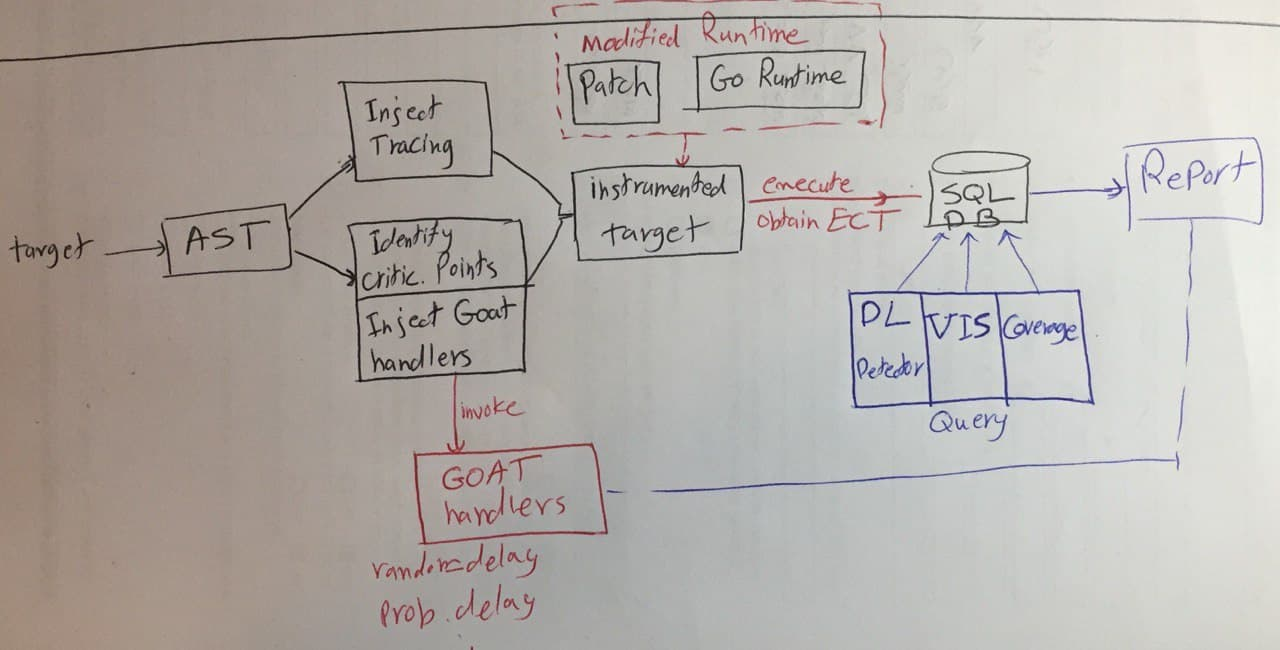
\includegraphics[width=.95\linewidth]{figs/overview-hand.jpg}
  \caption{Framework Overview}
  \label{fig:overview}
\end{figure}


\subsection{Execution Concurrency Tracing (ECT)}
\label{sec:ect}
When enabled, the execution tracer package captures and compresses an execution trace (ET).
%
Upon program termination, the ET is flushed to an IO buffer.
%
The decompressed ET is a sequence of events with a precise nanosecond-precision timestamp and a stacktrace for most events (total of 49 events \cite{goParserSource}, categorized and summarized in table \ref{tab:events}).
%
Through a one-time patch, we extend and enrich ETs with \textit{concurrency usage} events to obtain \textit{execution concurrency traces} (ECT):
\begin{itemize}
    \item \textbf{Channel:} For each channel operation (make, send, receive, close), ECT includes an event with the full stack trace of up to application source line number, a unique id to distinguish between different invocations (e.g., in a loop), and an argument to show the type of operation (blocking/non-blocking based on the state of channel buffer). Upon creation, a unique id is assigned to each channel to keep track of its operations during execution.
    \item \textbf{Mutex, WaitGroup \& Conditional Variables:} Similar to channels, we assign a unique id to each concurrency object and emit an event for each of their operations (lock, unlock, add, wait, signal, broadcast). We also distinguish between non-blocking operations (e.g., free mutex) and blocking ones.
    \item \textbf{Select \& Schedule:} The scheduler and the \textit{select} structure introduce non-determinism to the execution. We keep track of the decisions made by the scheduler and select statements to obtain an accurate \textit{decision path} during execution.
\end{itemize}

Having a precise model of concurrency primitives such as the ECT enables interesting analysis in offline space.
%
Valuable knowledge such as frequency of concurrency usage per goroutine, blocking/non-blocking execution of concurrency primitives, and the last event executed by each goroutine (for leak detection) can get extracted from ECT.


\begin{table}[b]
    \centering
        \begin{tabular}{|l|l|}
        \hline
        \rowcolor[HTML]{C0C0C0}
        \multicolumn{1}{|c|}{\cellcolor[HTML]{C0C0C0}\textbf{Category}} & \multicolumn{1}{c|}{\cellcolor[HTML]{C0C0C0}\textbf{Description}} \\ \hline
        Process & Indication of process/thread start and stop \\ \hline
        GC/Mem & Garbage collection and memory operation events\\ \hline
        Goroutine & Goroutines events: create, block, start, stop, end, etc. \\ \hline
        Syscall & Interactions with system calls \\ \hline
        Users & User annotated regions and tasks (for bounded tracing) \\ \hline
        Misc & System related events like futile wakeup or timers \\ \hline
        \end{tabular}

    \caption{Event categories by the Go execution tracer}
    \label{tab:events}
\end{table}



\subsection{Critical Points}
\label{sec:critical}

Through statically traversing the AST of any target package (e.g., files of the “main” package), goat gathers a set of line numbers where concurrency functions are used. These points (aka critical points) are the points where a context switch might drastically change the concurrency behavior of the program and trigger an undiscovered bug. Here are the AST nodes that represent a critical point:
Go: ast.Node GoStmt   (example: go func() // spawning a new goroutine)
Send: ast.Node SendStmt     (example: channel <- x)
Recv: ast.Node UniExprStmt(op=”<-”) (example:  <- channel)
Mutex, WaitGroup, CondVars: ast.Node CallExpr (example: xxx.Lock())
Xxx.Lock()
Xxx.Unlock()
Xxx.Add()
Xxx.Wait()
Xxx.Signal()
Xxx.Broadcast()
Careful adjustment is required for Select and Range statements that have send/recv as their children in the AST.

\subsection{Instrumentation}
\label{sec:instrument}
Identifying “critical points”:
Instrumentation: goat inject goat\_handler() calls before the critical point nodes. Goat\_handler() can be a call to any desired scheduler-manipulator. For instance, currently it calls an external function that randomly and boundedly yield to all other runnable goroutines (i.e., call gosched()). It gives us the flexibility to experiment different kinds of random and systematic (e.g., coverage-guided) scheduler-manipulation from an external function and environment variables without touching goat or goatlib API. In addition to critical points, goat adds four more line to the beginning of main function:
Import goat
goat\_done := goat.Start() // Start() initializes goat and starts tracing. It also creates and returns a channel for signaling the Stop()
go goat.Watch(goat\_done) // spawns a new goroutine as a watcher for liveness of the program (in case of global deadlocks or infinite loop). Watch() either receives from done and performs : goat\_done <- true, or timeouts and stop tracing, and terminates.
defer goat.Stop(goat\_done) // after the main ends, Stop() is called to send a value to the watcher goroutine and signaling that the program is finished. Then it waits to receive the ack from watcher, then stops tracing and terminates.
Trace collection: Currently, goat can collect a plain ECT from the native execution and also ECTs from executions with manipulated scheduler.
Deadlock detector: After the program terminates, goat queries the database to distinguish main goroutines and application spawned goroutines from background goroutines (runtime, tracing, etc.). Then it checks if all application goroutines ended with “GoEnd” (otherwise there is leak – partial deadlock) and if the main goroutine is ended with “GoSched” (otherwise there is a global deadlock since main did not finish).


\subsection{Deadlock Detection}
\label{sec:deadlock}

\begin{itemize}
  \item \textbf{Identifying Root, Main and App goroutines:}
  In the lifetime of a program, the runtime system creates new goroutines or pick from the pool of dead goroutines to perform various tasks such as bootstrapping the program, garbage marking and sweeping, and tracing.
  %
  \goat also adds extra goroutine to \textit{watch} the main goroutine in case of blockage of the main goroutine.
  %
  These extra goroutines are captured in the tracing but we are not interested in studying them as our main focus is the main application (or test) and all application-level goroutines.
  %
  By checking the stack of creation location, \goat prune the goroutine tree from unimportant goroutines.
  %
  We only keep and analyze events from the execution of main goroutine and all G such that ancestor(G) = main.
  \item \textbf{Final Event:}
  ECT captures end-to-end sequence of events for each goroutine representing its lifetime behavior.
  %
  If tracing is enabled, every application goroutine invokes the tracer to capture $GoEnd$ before finishing its execution and exit (change status from \textit{grunnable} to \textit{gdead})\cite{goexit-line-of-code}.
  %
  Before the main function returns (\ie exits), it calls the scheduler (through runtime.Gosched() invocation which captures $GoSched$ event) to hand over the control to the root goroutine to finish up program execution.
  %
  Since we instrument the application to stop tracing when main returns (through calling trace.Stop()), $GoSched$ would be the last event captured for the main goroutine if it returns succesfully.
  %
  We call an execution \textbf{successful}, if below conditions hold
  \begin{itemize}
    \item (1) all goroutines spawned in the main goroutine has $GoEnd$ as their final event
    \item (2) the final event of the main goroutine is $GoSched$ with \texttt{runtime.traceStop} on top of its stack.
  \end{itemize}
  If either of above conditions does not satisfy after program execution, a \textbf{deadlock} happens because it shows that there are one or more goroutine that did not reach its final state.
  %
  A one-line query to the application database retrieves the final event of each executed goroutine.
  %
    
\end{itemize}
